\documentclass[sigplan, review, screen, 10pt]{acmart}
\renewcommand\footnotetextcopyrightpermission[1]{}
\settopmatter{printfolios=false,printccs=false,printacmref=false}

\acmYear{2024}\copyrightyear{2024}
\acmConference[Brown 2952r'24]{Brown's Systems Transforming Systems}{Fall, 2024}{Providence, RI}
% \acmBooktitle{}
% \acmPrice{}
% \acmDOI{}
% \acmISBN{}

\usepackage{enumitem}
\usepackage{booktabs}
\usepackage{soul}
\usepackage{xspace}
\usepackage{color}
\usepackage{xcolor}
\usepackage{upquote}
\usepackage{listings}
\usepackage{amsmath}
\usepackage{wrapfig}
\usepackage{syntax}
\usepackage{caption}
\usepackage{picins}
\usepackage{minted}

\newcommand{\eg}{{\em e.g.}, }
\newcommand{\ie}{{\em i.e.}, }
\newcommand{\etc}{{\em etc.}\xspace}
\newcommand{\vs}{{\em vs.} }
\newcommand{\cf}[1]{(\emph{Cf}.\S\ref{#1})}
\newcommand{\sx}[1]{(\S\ref{#1})}
\newcommand{\sys}{{\scshape pSys}\xspace}

\renewcommand{\shortauthors}{J. S. Carberry}

\bibliographystyle{ACM-Reference-Format}

\usepackage{booktabs}
\usepackage{subcaption}

\title{sysX: A new technique or system}

\author{Josiah Stinkney Carberry}
\affiliation{Brown University}
\email{jcarb@brown.edu}

\begin{document}

\begin{abstract}
This paper presents the design, implementation, and evaluation of sysX, a new something something
\end{abstract}

\maketitle

% \pagestyle{plain}

\section{Introduction}
\label{intro}

This sentence confirms that citations work~\cite{kpn74, dryad07}. Provide
context etc.

The paper is structured as follows.
It starts by introducing the necessary background on/example of using \sys~\sx{bg}.
Sections \ref{one}--\ref{three} highlight key contributions:
\begin{itemize}
	\item
	\S\ref{one}
		outlines a section and contribution.

	\item
	\S\ref{two} outlines another section and contribution.

	\item
	\S\ref{three} is similar about \sys's third contribution and a corresponding section.

\end{itemize}

\noindent
After \sys's evaluation~\sx{eval} and  comparison with related work~\sx{related}, the paper concludes~\sx{discussion}.  

\begin{figure}[t]
\centering
% https://docs.google.com/drawings/d/1yYUWsfreEDoHUXxcIAF62bnzgahHs76YQwM9vbmVkgA/edit?usp=sharing
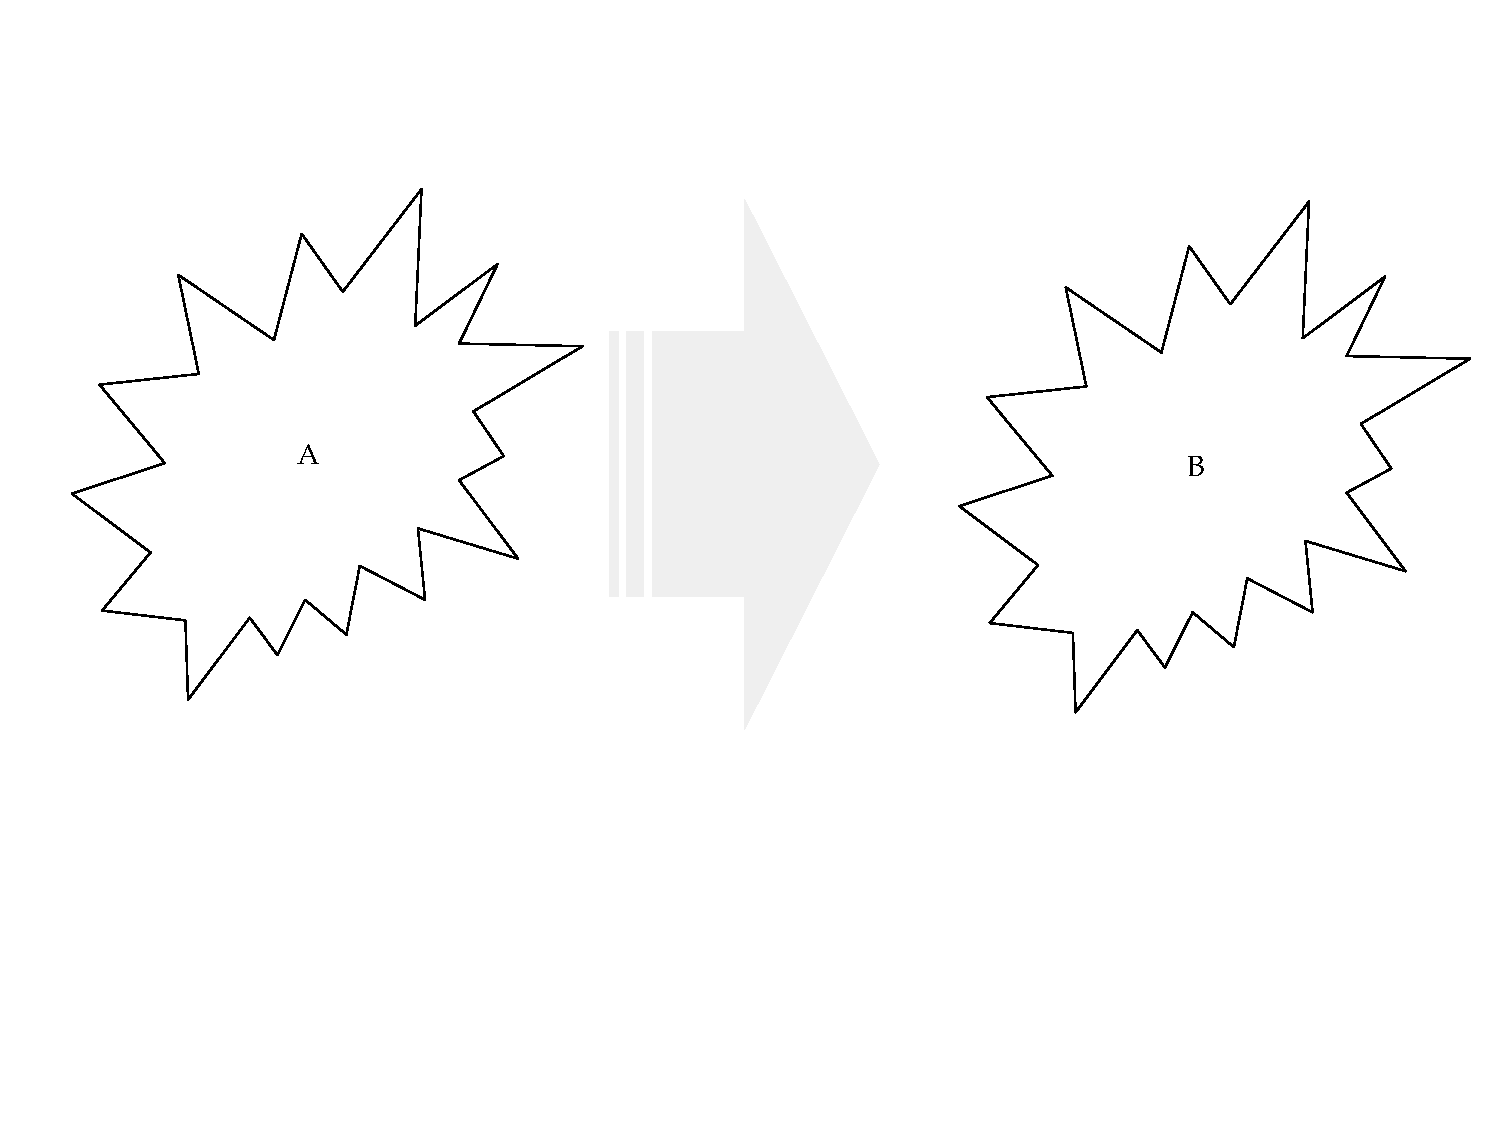
\includegraphics[width=0.49\textwidth]{./figs/cs2952r.pdf}
\caption{
  \textbf{\sys overview.}
  ..and an overview description
}
\vspace{-18pt}
\label{fig:overview}
\end{figure}

\section{Background, Example, \& Overview}
\label{bg}

This section ...

\subsection{Running Example: Searching for Patents}
\label{bg:patents}

\textbf{An Example} Walk the reader through an example

\begin{figure}[t]
\centering
\begin{minted}[fontsize=\footnotesize]{javascript}
// this is an example of a code snippet
import { createServer } from 'node:http';
const server = createServer((req, res) => {
  res.writeHead(200, { 'Content-Type': 'text/plain' });
  res.end('Hello World!\n');
});
// starts a simple http server locally on port 3000
server.listen(3000, '127.0.0.1', () => {
  console.log('Listening on 127.0.0.1:3000');
});
\end{minted}
\caption{
  \textbf{Server example}
  This snippet shows how to use minted to demonstrate code.
}
\label{fig:example}
\end{figure}

\subsection{Design Overview}

\label{bg:overview}

\section{Technical Section 1}
\label{one}

\section{Technical Section 2}
\label{two}

\section{Technical Section 3}
\label{three}

\begin{table}[t]
\center
\footnotesize
\setlength\tabcolsep{3pt}
\caption{
    \textbf{Component decomposition}.
    The table below summarizes some information
}
\begin{tabular*}{\columnwidth}{l @{\extracolsep{\fill}} llll}
\toprule
Component          &  C     & Description & 1             & Something   \\
\midrule
component 1        & 2      & Mini        &  13 (12.5\%)  & else        \\
component another  & Joseph & Mini        &  17 (16.3\%)  & else        \\
\bottomrule
\vspace{-18pt}
\end{tabular*}
\label{tab:components}
\end{table}

\section{Evaluation}
\label{eval}

\section{Discussion}
\label{discussion}


\section{Related Work}
\label{related}

\section{Conclusion}
\label{conclusion}

The system's implementation, as well as all the example code and benchmarks presented in this paper, are all open source and available for download:
\href{https://github.com/something/else}{github.com/something/else}.

% \subsection*{Acknowledgements}
\begin{acks}

\end{acks}

%% Bibliography
{\small
\bibliography{./bib}
}

\appendix

\section{Using our System}
\label{using-apx}

The section below summarizes how to deploy and use our system..

\end{document}

